\section{Support Vector Machine and Structured Learning}

\begin{frame}{Structured Problems}
    \begin{itemize}
          \item Do not predict single value, but a structured object,
        \begin{itemize}
              \item[] \eg predict a path
        \end{itemize}
          \item Utilize structured loss for a better evaluation of prediction, 
        \begin{itemize}
              \item[] \eg quantize prediction error for tracking based on a tree comparison of lineages rather than 1-0 loss for single event matches
        \end{itemize}
    \end{itemize}
\end{frame}g


\begin{frame}{Structured Problem - Path Prediction}
    PUT IMAGE HERE!!
\end{frame}


\begin{frame}{Support Vector Machines - Prediction}
    \begin{itemize}
          \item linear two-class classifier
          \item score input $\textbf{x}$ and assign label according to sign of score
        \begin{itemize}
              \item[] $y_{\text{predict}} = \sgn\left(\textbf{w}^{\intercal}\textbf{x} + b\right)$
        \end{itemize}
          \item parameters $\textbf{w}$, $b$ determined by training
    \end{itemize}
\end{frame}


\begin{frame}
    \frametitle{Support Vector Machines - Training }
    \begin{itemize}
          \item minimize regularized cost function
          \item[] \begin{align}
            &\textbf{w}^*, b^*  = \argmin_{\textbf{w}, b} \frac{1}{2} \textbf{w}^{\intercal} \textbf{w}
            + \frac{C}{kN}\sum_{n=1}^N\left(\xi_n\right)^k \\
            &\phantom{\textbf{w}^*, b^*  = }\st \nonumber \\ 
            &y_n\left(\textbf{w}^\intercal\textbf{w}+b\right) \geq 1 - \xi_n \; \forall n \in \{l \in
            \mathbb{N} | l < N\}
        \end{align}
          \item typically, $k\in\{1,2\}$
        \item \fullcite{barber_12_bayesian} for more details
    \end{itemize}
\end{frame}


\begin{frame}
    \frametitle{Support Vector Machines - Two Class Example}
    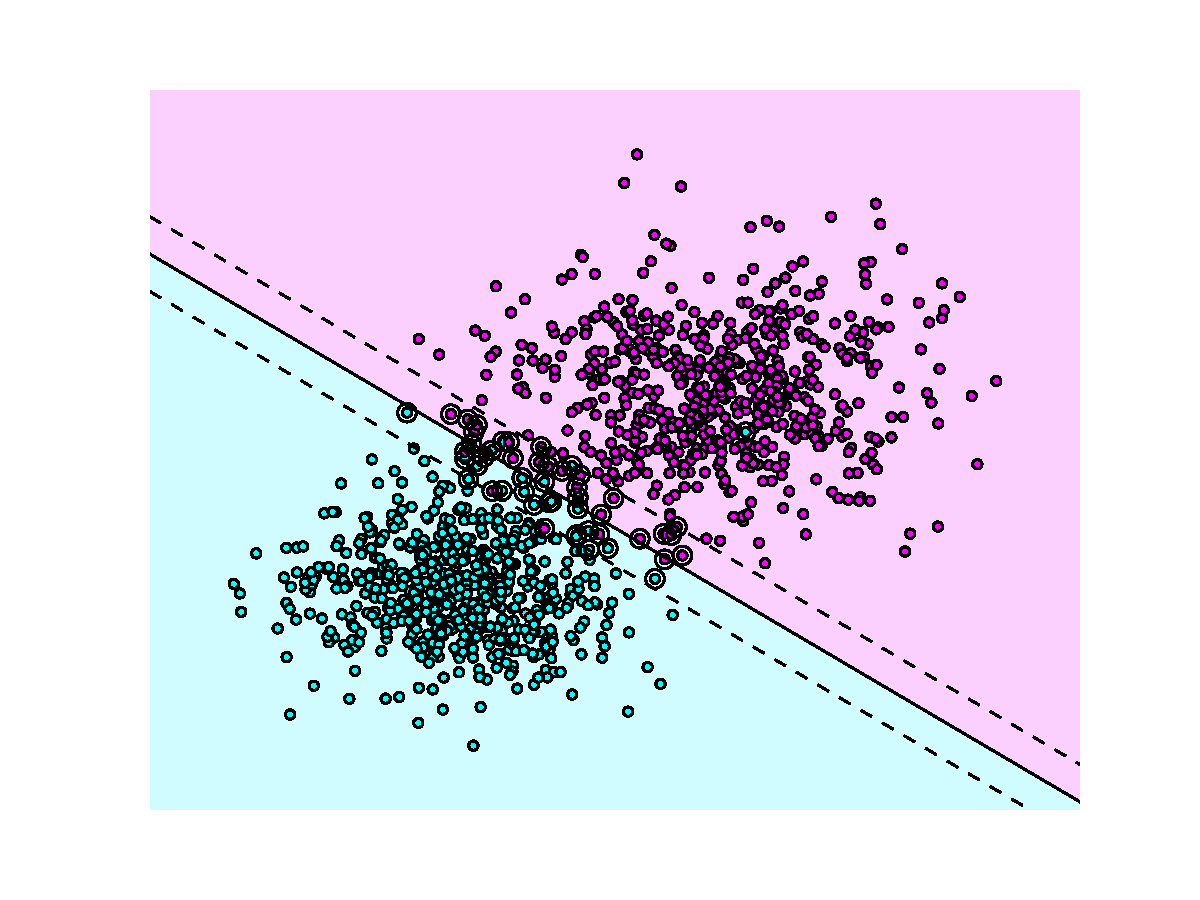
\includegraphics[width=\textwidth]{images/two_class_svm.pdf}
\end{frame}


\begin{frame}
    \frametitle{From Single/Two Class to Multi Class}
    \begin{itemize}
          \item Introduce one SVM classifier ($\textbf{w}_y, b_y$) for each class $y$
          \item For prediction, the maximum scoring classifier determines the label
        \begin{itemize}
              \item[] $\displaystyle y_{\text{predict}} = \argmax_y \;
            \bigl(\left(\textbf{w}_y\right)^{\intercal}\textbf{x} + b_y\bigr) $
        \end{itemize}
    \end{itemize}
\end{frame}


\begin{frame}
    \frametitle{Support Vector Machines - Three Class Example}
    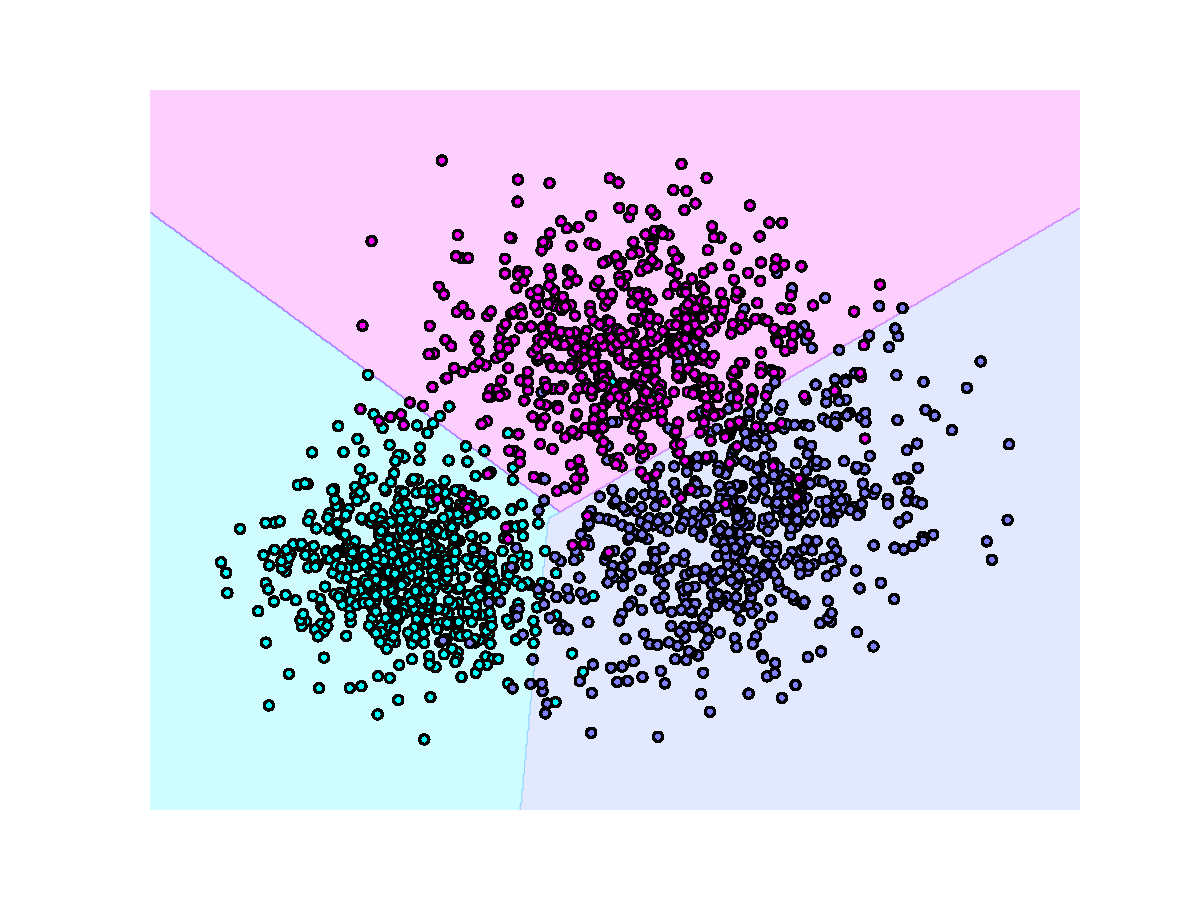
\includegraphics[width=\textwidth]{images/three_class_svm.pdf}
\end{frame}

\begin{frame}
    \frametitle{From SVM to Structured Learning}
    \footfullcite{joachims_04_support}
\end{frame}


%%% Local Variables: 
%%% mode: latex
%%% TeX-master: "../main"
%%% End: 
